% !TeX root = report.tex
\documentclass{ctexart}

\usepackage{tikz}
\usetikzlibrary{3d}

\usepackage{hyperref}

\title{六自由度机械臂系统建模分析}
\author{***REMOVED*** \\ ***REMOVED***}

\begin{document}

\maketitle

\section{问题简述}

随着工业自动化的大规模发展,机械臂在生产中得到了大规模的使用。
在众多机械臂中,三自由度机械臂凭借结构简单、控制容易以及造价低廉等优势受到青睐,因此也成为重要的研究对象。

本技术报告将对一个经典的三自由度机械臂以及机械臂末端安装的三自由度机械手进行运动学分析、动力学分析和控制仿真。
该机械臂总共具有六个自由度,能够在三维空间中自由运动,实现指定的目标。

\subsection{机械臂模型}

\begin{figure}[ht]
    \centering
    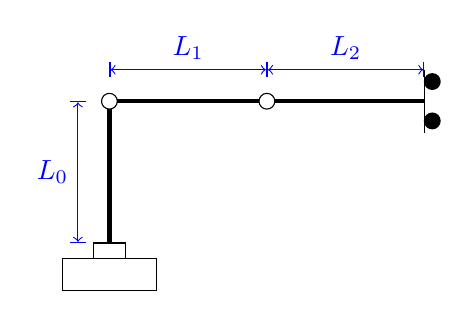
\begin{tikzpicture}
        % Arm 1 and foundation
        \draw (0.6, 0) rectangle (-0.6, -0.4);
        \draw (0.2, 0.2) rectangle (-0.2, 0);
        \draw [ultra thick] (0, 0.2) -- (0, 2);

        % Arm 2 and joint
        \draw [ultra thick] (0, 2) -- (2, 2);
        \draw [fill=white] (0, 2) circle [radius=0.1];
        
        % Arm 3 and joint
        \draw [ultra thick] (2,2) -- (4,2);
        \draw [fill=white] (2,2) circle [radius=0.1];
        \draw (4, 1.6) -- (4, 2.4);
        \draw [fill=black] (4.1, 1.75) circle [radius=0.1];
        \draw [fill=black] (4.1, 2.25) circle [radius=0.1];

        % Annotations
        \draw [|<->|, blue] (-0.4, 0.2) -- (-0.4, 2) node [pos=0.5, left] {$L_0$};
        \draw [|<->|, blue] (0, 2.4) -- (2, 2.4) node [pos=0.5, above] {$L_1$};
        \draw [|<->|, blue] (2, 2.4) -- (4, 2.4) node [pos=0.5, above] {$L_2$};
    \end{tikzpicture}
    \caption{机械臂主体部分示意图}
    \label{fig:robotic-arm-schema}
\end{figure}

本报告研究的机械臂系统由两个部分组成,第一个部分为具有三个旋转关节的三自由度机械臂,能够实现较大范围的自主运动;
第二个部分为机械臂末端安装的机械手型装置,该手型装置也具有三个自由度,能够实现对手持仪器的紧密操作。
该机械手型装置可视为一个三自由度关节,也视为三个紧邻的单自由度关节。
由于机械手的质量相对于机械臂主体可忽略,在动力学分析中可以不对后三个关节进行建模。
机械臂主体部分的示意图见图\ref{fig:robotic-arm-schema}。

\section{运动学模型}

我们使用机器人学中广泛应用的\emph{Denavit-Hartenberg 方法}为每一个关节分配固连坐标系并进行运动学分析,分配的坐标系如图\ref{fig:affixed-frame}所示。

\begin{figure}[ht]
    \centering
    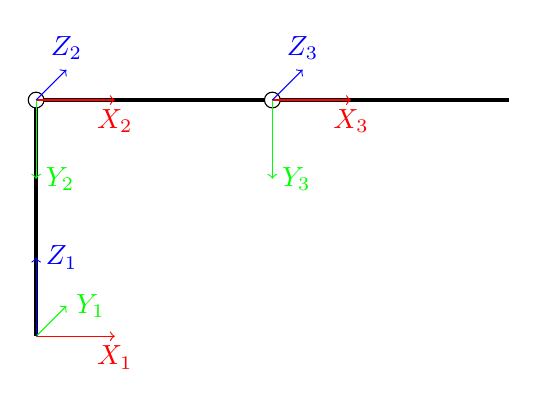
\begin{tikzpicture}
        % Arm 1
        \draw [ultra thick] (0, 0) -- (0, 3);

        \draw [->, red] (0,0,0) -- (1,0,0) node [below] {$X_1$};
        \draw [->, green] (0,0,0) -- (0,0,-1) node [right] {$Y_1$};
        \draw [->, blue] (0,0,0) -- (0,1,0) node [right] {$Z_1$};

        % Arm 2
        \draw [ultra thick] (0, 3) -- (3, 3);
        \draw [fill=white] (0, 3) circle [radius=0.1];
        \draw [->, red] (0,3,0) -- (1,3,0) node [below] {$X_2$};
        \draw [->, green] (0,3,0) -- (0,2,0) node [right] {$Y_2$};
        \draw [->, blue] (0,3,0) -- (0,3,-1) node [above] {$Z_2$};

        % Arm 3 and joint
        \draw [ultra thick] (3,3) -- (6,3);
        \draw [fill=white] (3,3) circle [radius=0.1];
        \draw [->, red] (3,3,0) -- (4,3,0) node [below] {$X_3$};
        \draw [->, green] (3,3,0) -- (3,2,0) node [right] {$Y_3$};
        \draw [->, blue] (3,3,0) -- (3,3,-1) node [above] {$Z_3$};
        
    \end{tikzpicture}
    \caption{固连坐标系分配}
    \label{fig:affixed-frame}
\end{figure}

按照指定的方法分配每个关节的固连坐标系后,可得出每个关节的 Denavit-Hartenberg 参数,如表\ref{tab:DH-params}所示。

\begin{table}[ht]
    \caption{Denavit-Hartenberg参数}
    \label{tab:DH-params}
    \centering
    \begin{tabular}{c|cccc}
        \hline
        & $\alpha_{i-1}$ & $a_{i-1}$ & $d_i$ & $\theta_i$ \\
        \hline
        1 & $0$ & $0$ & $0$ & $\theta_1$ \\
        2 & $-\frac{\pi}{2}$ & $L_1$ & $0$ & $\theta_2$ \\
        3 & $0$ & $L_2$ & $0$ & $\theta_3$ \\
        4 & $-\frac{\pi}{2}$ & $L_3$ & $0$ & $\theta_4$\\
        5 & $\frac{\pi}{2}$ & $0$ & $0$ & $\theta_5$\\
        6 & $-\frac{\pi}{2}$ & $0$ & $0$ & $\theta_6$\\ \hline
    \end{tabular}
\end{table}

\subsection{逆向运动学}

\section{动力学模型}

\section{控制器设计与仿真}

\end{document}
